
\chapter{Blockchain}
Consensus protocols that work with Byzantine-failure nodes and allow open membership is used in open blockchains. By open blockchain, we understand the blockchains where nodes can freely join the network and participate in the consensus protocol. Examples of such blockchains are Bitcoin, Ethereum, and Stellar. Bitcoin uses a proof-of-work consensus algorithm where the computational power dictates the contribution to the consensus decision. Ethereum plans to switch to a proof-of-stake consensus where the amount of cryptocurrency dictates the contribution to the consensus decision. Stellar uses federated byzantine agreement where the trust dictates the contribution to the consensus decision. Data stored in Blockchain is immutable, transparent, and secure. Data types differ in different blockchains, but most of them store the transactions that update the global ledger. Some blockchains, like Ethereum, also allows storing smart contracts\footnote{Scripts that are executed on virtual machines on all nodes and uses blockchain as a persistent storage}. In our case, we use blockchain to store proofs-of-time claims. Fortunately, such claims can be embedded in most of the blockchains data types.

Let's imagine a naive solution based on the Bitcoin blockchain. The solution is naive because proof-of-work has no practical application in our system. We can not base our system on the competitive consensus algorithms, especially on resource-constrained network devices. Nevertheless, the solution can be applied to any other consensus protocol, so we decide to explain it on the simplest and most commonly known one. 
Before we start to explain the algorithm, let's recall what we want to achieve. We want the end-user, the content consumer to be sure about the content authentication. We achieve it by requiring the publisher to prove its access to private keys for a long period of time, long enough so the malicious publisher can not afford to do that, while legit publisher can. We call those access proofs––proofs-of-time. In the GI algorithm, the proof-of-time is denoted in a sequential number of external infections. The publisher who can perform long enough proof-of-time can create strong initial power of chain reaction, that will lead to an epidemic, while the weak proof-of-time will eventually lead to extinction. 

In the blockchain solution, the simplest way to proof access to private-key in the context of some content is to publish transactions from the publisher account to the content account. The content account is the imagined account whose address is the hash of such content. The publisher's account is the same key-pair used to sign the content in the ICN network. The flow is shown in Fig. \ref{fig:distribution-flow}.
\begin{figure}[h!]
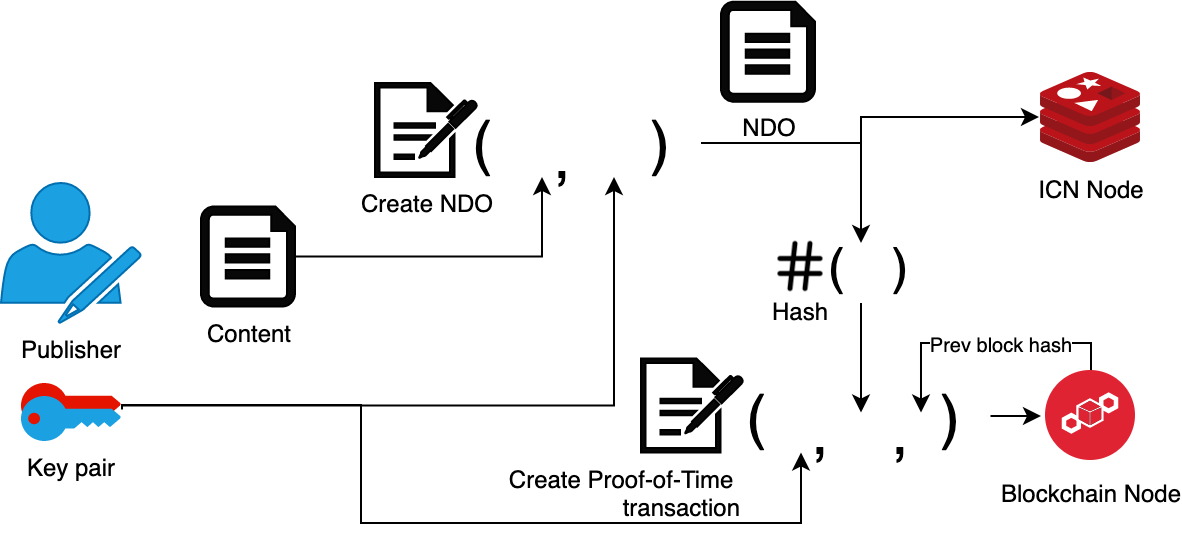
\includegraphics[width=9cm]{img/distribution-flow.png}
\centering
\caption{Flow of publishing content to ICN and proof-of-time to blockchain}
\label{fig:distribution-flow}
\end{figure} 
The strength of the proof-of-time is calculated by counting the total number of transactions to the content hash address. 
Here we will use one of the most fundamental features in Bitcoin blockchain––blocks. Block is a container holding bunch of transactions. Bitcoin is designed to produce a new block every 10min on average, it is achieved by the dynamic complexity of the mining process. If we count each block where the transaction from the publisher account to the content hash exists, we get the strength of proof-of-time that can be interpreted as sufficient to trust the content. This way, the proof-of-time is propagated not as a consensus, but as an overlay structure on top of a trusted immutable database. In Figure \ref{fig:claims-structure} we show an example of three blocks consisting of proof-of-time claims. Each block also consists of some meta-data like a hash of its content, a hash of the previous block (pointer to the previous block), and block creation timestamp. We assume that blocks are created with 10min intervals, and each content requires proof-of-time in minimum strength of 20min. Alice first publishes her content to the ICN node getting the hash of the NDO as shown in Figure \ref{fig:distribution-flow}, then the claim is created and published to the Blockchain node. After 10 minutes once again she publishes the claim, and again after another 10 minutes she repeats the process. Three publications in a row certify that Alice had Alice's credentials for at least 20min. Bob was able to publish only two claims, which we consider not enough to trust the content. Carol, on the other hand, skipped the second block which is considered as a break in the proof-of-time chain, therefore we start measuring the proof-of-time from the third block.
The user who wants to determine if the content is authenticated can just ask the Blockchain node about all the transactions that were sent to the content-hash-account, and validate if there exists enough number of claims from the content publisher. 
The mechanism can be extended to the "certification services" (discussed in chapter \ref{mitigating-certification-services}) in such a way that not only the publisher can participate in creating proof-of-time claims, but also some set of trusted units that can certify the content trustworthy–––similar how we trust root CA certificates. 
\begin{figure}[h!]
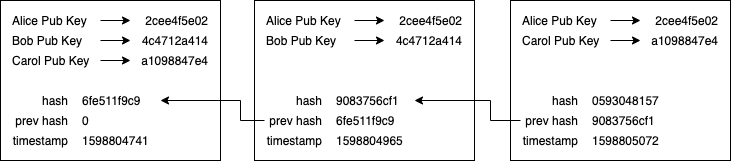
\includegraphics[width=\textwidth]{img/claims-structure.png}
\centering
\caption{Claims structure in blockchain}
\label{fig:claims-structure}
\end{figure} 

As we mentioned earlier, the Bitcoin consensus protocol and any other Nakamoto Consensus––in which the leader capable of updating the blockchain is elected in form of lottery where the chance of winning is determined by the amount of spent resource––is not suitable for our use case. Fortunately, the topic of distributed systems and especially consensus algorithms are studied for decades so there is a lot to choose from.

\section{Federated Byzantine Agreement}
\label{FBA}
We find Federated Byzantine Agreement (FBA)––and its blockchain Stellar Consensus Protocol (SCP)\cite{mazieres2015stellar}––the most suitable protocol for our needs. In contrast to proof-of-work, where computational power dictates the contribution to consensus, FBA is based on a trust model. That way, it becomes a fast, lightweight, and asymptotic resistant\footnote{the node consisting of large computational power does not gain any advantages in the consensus protocol}. Instead, the contribution value is determined by the node trustworthy––similar to GI protocol. A new node, joining the network, has no contribution to the protocol until someone trusted––start to trust it.
Blockchain like any other asynchronous distributed system faces FLP\cite{fischer1985impossibility} impossibility trilemma––where only two of three properties can be achieved. Those properties are Fault tolerance, Liveness, and Safety. Most systems must be fault tolerance so the choice is left between Liveness and Safety. Safety guarantee state consistency across all nodes in the network. If nodes do not agree on some transaction, they will not split into two different states, but rather wait until the conflict is resolved. Liveness guarantee that the consensus will always terminate and the system will always be available to accept new transactions. When the conflict occurs, the ledger is split into two different versions, until it's resolved, but in the meantime, it can process new transactions. Most of the blockchain protocols choose liveness, tolerating temporary partitioning. They argue that the time of the partitioning is short enough that the users expecting high credibility of the transaction can just wait---until the chance of shifting the state is acceptably small\footnote{In proof-of-work the chance of changing the state of some block gets smaller with the length of the chain of the blocks attached to this block}. The conflict settlement is dictated, again, by computational power. The state which gets the fastest used as a previous block is considered the winner. That way the system can guarantee permanent availability, even with just one working node. 

Stellar Consensus Protocol on the other hand chooses Safety over Liveness. Once the state has been approved, it can not be changed. State gets approved when the quorum of the network agree on the proposed state. This allows much faster confirmation times, in Stellar the ledger closes in about 5 sec. 
Stellar Consensus Protocol is based on Practical Byzantine fault tolerance (PBFT)\cite{castro1999practical}, and extends its functionality by allowing open membership, therefore promoting decentralization. In SCP each node pick its trusted set of nodes called \textit{quorum slice} (in which it is also \textit{ipso facto} a member). The \textit{quorum slice} should be different for each node, but naturally, some nodes are more trustworthy, therefore are chosen more often in the quorum slices. Transitive trust for all node's \textit{quorum-slice} members, forms \texit{quorum}. For any two quorums, there must exist \textit{quorum-intersection} to prevent network partitioning. 

In non-federated byzantine agreement systems, the decision on some state proposal is determined by the majority of the nodes. Once the proposal gets accepted by a quorum (a majority of the nodes), the rest of the network can be sure that other proposals will fail, since they can't reach the quorum, since the nodes can't change their mind. That way the whole network converges to the final outcome.
In decentralized systems, where nodes can join and leave at will, it is hard to know the total number of nodes in the network \texit{a priori}. Therefore it's hard to calculate the majority of the network. Additionally, open systems can not rely on quantitive majority since this would open them to Sybil attacks\footnote{In this attack single entity can join many nodes to the network that looks as independent units, therefore forcing decisions based just on the majority number of nodes}. To solve this issue, FBA introduces the federated voting process that starts locally and expands until it reaches the whole network. To make it work, the local quorums must overlap with at least one node that will convey the voting decisions across different quorums. This property guarantee that if one quorum agrees on some value P, the other quorum can not agree on not-P, because it includes some nodes from the first quorum that already voted on P.

Federated voting starts when some node sends a broadcast to the network announcing a vote on a particular value V. Node sending such value promise that it will never vote against V. Each node sees how other nodes are voting by their broadcast messages. If the node notice that some quorum of nodes voted on value V, it can be sure that such value will be eventually accepted by the whole network (by the definition of quorum), therefore it can switch to \textit{accepting V} state and announce that fact to the whole network, the same way as announced vote decision. Accepting is stronger than voting because voting for V means that the \textit{node} will never vote for non-V while accepting V means that the \textit{each node in the network} will never accept non-V. When a node notices some quorum of nodes accepting V, it \textit{confirms V}, and by the definition of the quorum, all nodes in the network will eventually confirm value V, ending the process of federated voting.

The problem arises, when such nodes which are in quorum intersection are Byzantine-failed, lying about the decisions made on each quorum. In SCP whitepaper, there is an assumption that the network is configured in such a way that even if the malicious nodes are removed from the network, it still holds quorum-intersection. If it does not hold, the network halts until the quorum-slices are reconfigured.
We can only \textit{expect} the network to form connections where there always exist quorum-intersection because the internet––that we are designing the protocol for––itself satisfy such property.

Another problem in an attempt to apply FBA to our use case might be the problem of the DoS attack. A malicious client might publish a huge number of proof-of-time claims successfully leading to network congestion. Stellar prevents that by introducing the transaction fees, therefore attacker is discouraged by financial means. Here in our approach, we don't want to introduce any financial aspects, so other mechanisms must be used to prevent it. DoS is a vital problem in ICN networking in general\cite{gasti2013and}, so the solutions that will be worked out will also solve our problems. 

There are several different blockchain consensus protocols, but not all of them are suitable for internet level protocol and to be run on network devices.
If we consider network devices similar to IoT devices we can leverage the research done on this kind of protocols \cite{salimitari2018survey}. The paper suggests that Stellar consensus is not ideal for IoT devices since it is too slow.
Since the proof-of-time claims are not the matter for milliseconds, but rather minuter or hours, we believe that the protocol is fast enough for our needs.
Also, there already exists a proposal of a modified FBA algorithm\cite{FCPpdf50:online} that uses a virtual voting algorithm that can achieve consensus in almost no communication overhead. We find this topic interested, and plan to research it in future work.

In this paper, the authors suggest that there is a subset of protocols especially suitable for IoT networks. Those protocols are Proof of Elapsed Time (PoET), Practical Byzantine Fault Tolerance (PBFT), and Tangle.

\section{Credibility Score}
In the GI algorithm, there are two states of content authenticity: authenticated or not-authenticated. We believe that this is limiting. Content like e.g. weather forecasting should not be authenticated for the same amount of time as an online banking website. Therefore we propose a more flexible model, where authentication can be acquired progressively via Credibility Score. Credibility Score mentioned in Section \ref{proof-of-time} increase authentication granularity. Pictures, music, movies don't require as much trust as websites where we enter our credentials and credit card details. Different thresholds should be used for different content types. For example, if 3 trust thresholds are used: low, medium, high; then we can require 10min, 2h, 12h of proofs of time accordingly. Each time the content is published to the network the author can be notified about that fact, and if the publisher used stolen credentials, the actual author has a time frame to revoke the credentials and halt the malicious authentication process.

\section{Blockchain layer}
In our proposition nodes in the network plays two roles, an ICN node where it participates in routing and content caching, and as blockchain node where he participates in consensus and blockchain storage (see Fig. \ref{fig:layers}a). Not every node has to play two roles, the ones which are not connected to end-uses might not participate in the blockchain network, since they don't get asked for content trustworthy. 
The blockchain layer could also be managed by completely different entities, separating the transport layer from the trust layer (see Fig. \ref{fig:layers}b). That way the ICN nodes could be abstracted from the trust network overhead introduced by the trust system––keeping them simpler. Also, the trust system would be more portable, it could be used in many different ICN solutions, and even in legacy systems since the trust does not depend on ICN, but on the hash of the content and publisher credentials. That way the blockchain trust network could be hosted by more powerful devices and possible different organizations––achieving separation of concerns which is always a good thing in the long term.

\begin{figure}[h!]
  \subfloat[Combined layers]{
	\begin{minipage}[c][1\width]{
	   0.5\textwidth}
	   \centering
	   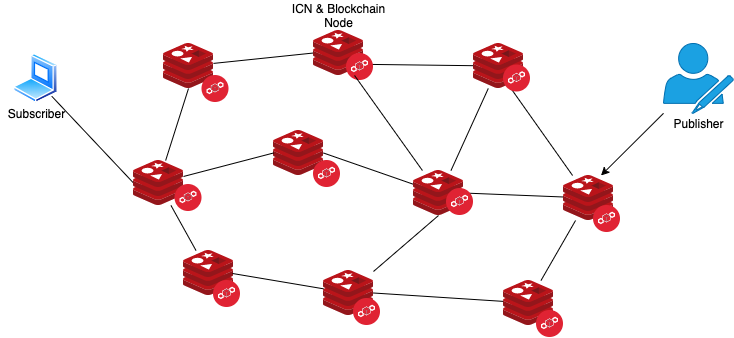
\includegraphics[width=1\textwidth]{img/combined-layers.png}
	\end{minipage}}
 \hfill
  \subfloat[Separated layers]{
	\begin{minipage}[c][1\width]{
	   0.5\textwidth}
	   \centering
	   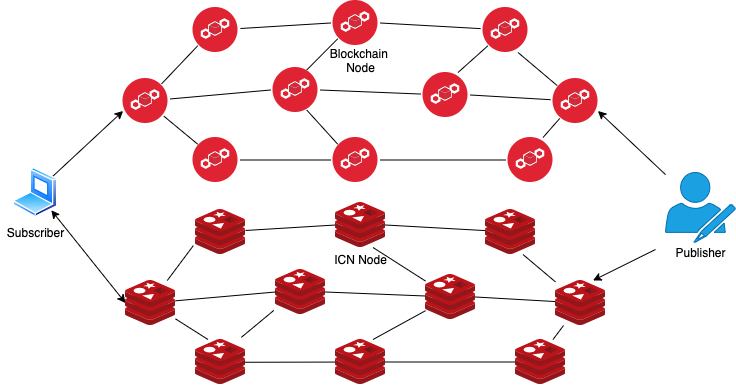
\includegraphics[width=1.1\textwidth]{img/separated-layers.png}
	\end{minipage}}
\caption{Layers}
\label{fig:layers}
\end{figure}

\section{Transaction throughput}
Transaction throughput––measured in transactions per second––is one of the biggest problem in blockchain ecosystem. Bitcoin public network can process up to 7 transactions per second (TPS), Ethereum can process 15TPS and Stellar can process 200TPS. The limitation comes from practical aspects of the system. 
\begin{enumerate}
    \item If we want the system to be decentralized, we can not require all nodes in the network to be super-computers, both in processing power and storage capacity. 
    \item If we want system to be scalable, it must be able to handle more TPS, than each single node can doprocess.
    \item If we want system to be secure, it must be tolerante attackers with   able to handle more TPS, than each single node can process.
\end{enumerate}
In our case, we design the system for network devices that have limited resources. Each node level we must allow as much devices as possible   Blockchain as a public decentralized system should be able to operate on

\section{Pruning Database}
Storing whole blockchain database can be very resource expensive. To 
